\documentclass[tikz,border=10pt]{standalone}
\usepackage{amsmath,amssymb}
\usetikzlibrary{calc,decorations.markings,fadings,shadings,arrows.meta,patterns}

\definecolor{NavyDeep}{HTML}{0F172A}
\definecolor{BlueCore}{HTML}{1D4ED8}
\definecolor{BlueMid}{HTML}{3B82F6}
\definecolor{BlueLight}{HTML}{93C5FD}
\definecolor{BlueGhost}{HTML}{DBEAFE}
\definecolor{TealAccent}{HTML}{0D9488}
\definecolor{SlateGray}{HTML}{64748B}

\begin{document}
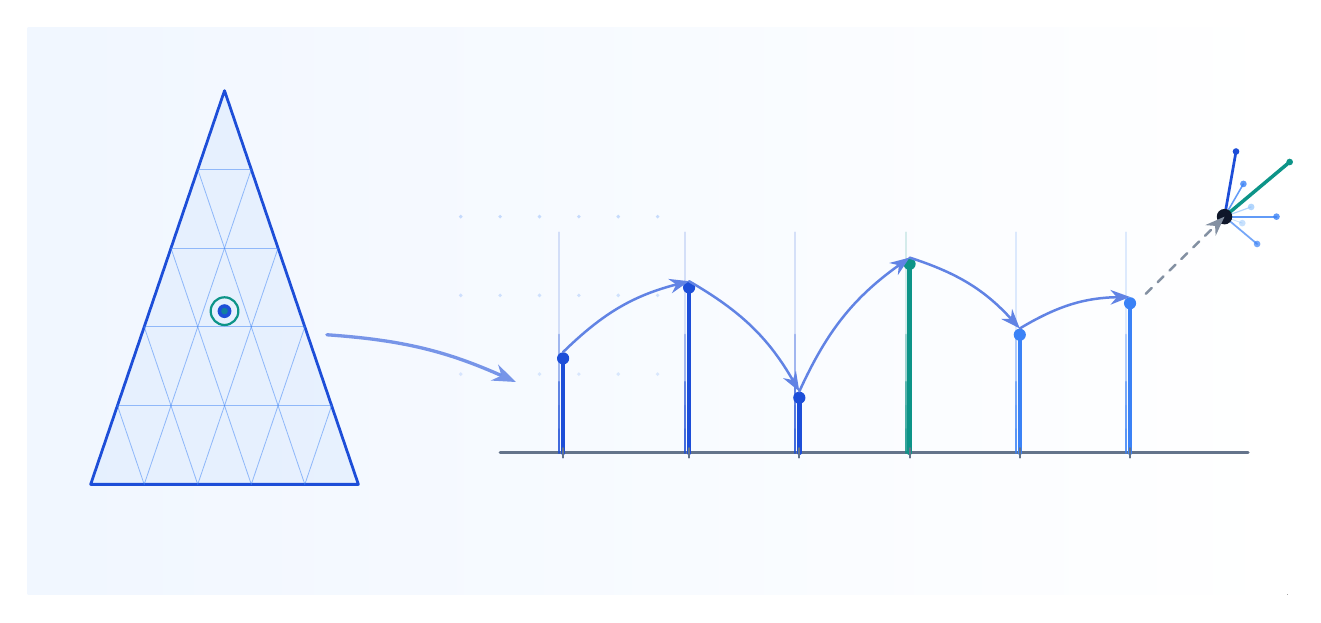
\begin{tikzpicture}[
  remember picture,
  line cap=round, line join=round,
  >=Stealth
]

% === Background gradient rectangle ===
\fill[left color=BlueGhost!40, right color=white] (-8,-3.6) rectangle (8,3.6);

% === Probability simplex (triangle) in the left ===
% Vertices of 3-simplex projection
\coordinate (S0) at (-5.5, 2.8);
\coordinate (S1) at (-7.2,-2.2);
\coordinate (S2) at (-3.8,-2.2);

\fill[BlueGhost, opacity=0.5] (S0) -- (S1) -- (S2) -- cycle;
\draw[BlueCore, line width=1.0pt] (S0) -- (S1) -- (S2) -- cycle;

% Simplex grid lines
\foreach \t in {0.2,0.4,0.6,0.8} {
  \draw[BlueMid, line width=0.3pt, opacity=0.5]
    ($(S0)!\t!(S1)$) -- ($(S0)!\t!(S2)$);
  \draw[BlueMid, line width=0.3pt, opacity=0.5]
    ($(S1)!\t!(S0)$) -- ($(S1)!\t!(S2)$);
  \draw[BlueMid, line width=0.3pt, opacity=0.5]
    ($(S2)!\t!(S0)$) -- ($(S2)!\t!(S1)$);
}

% Barycentric point (probability distribution)
\coordinate (P0) at ($(S0)!0.3!(S1)!0.5!(S2)$);
\coordinate (P0) at (-5.5,-0.0);
\fill[BlueCore] (P0) circle (2.5pt);

% === Autoregressive chain: sequence of probability spikes ===
% Represent tokens as vertical "spikes" on a timeline
\def\tbase{-1.8}
\def\tymax{2.8}
\def\tystep{0.5}

% Timeline base
\draw[SlateGray, line width=1.0pt] (-2.0,\tbase) -- (7.5,\tbase);

% Token positions
\foreach \x/\h/\col in {
  -1.2/1.2/BlueCore,
   0.4/2.1/BlueCore,
   1.8/0.7/BlueCore,
   3.2/2.4/TealAccent,
   4.6/1.5/BlueMid,
   6.0/1.9/BlueMid%
}{
  % Distribution bars behind
  \foreach \bh/\bo in {0.3/0.08, 0.6/0.05, 0.9/0.12, 1.5/0.07, 2.8/0.04} {
    \draw[\col, line width=0.8pt, opacity=\bo*4]
      (\x-0.05, \tbase) -- (\x-0.05, \tbase+\bh);
  }
  % Main spike
  \draw[\col, line width=1.6pt]
    (\x, \tbase) -- (\x, \tbase+\h);
  \fill[\col] (\x, \tbase+\h) circle (2.2pt);
  % Tick mark
  \draw[SlateGray, line width=0.7pt] (\x, \tbase-0.06) -- (\x, \tbase+0.06);
}

% Autoregressive arrows connecting peaks
\foreach \xa/\xb/\ha/\hb in {
  -1.2/0.4/1.2/2.1,
   0.4/1.8/2.1/0.7,
   1.8/3.2/0.7/2.4,
   3.2/4.6/2.4/1.5,
   4.6/6.0/1.5/1.9
}{
  \draw[BlueCore!70, line width=0.9pt, ->, bend left=15]
    (\xa, \tbase+\ha+0.08) to (\xb, \tbase+\hb+0.08);
}

% === Softmax "fan" on the right of the chain: next-token distribution ===
\coordinate (fan) at (7.2, 1.2);
\foreach \ang/\len/\col/\opa in {
  80/1.4/BlueCore/1.0,
  60/0.8/BlueMid/0.8,
  40/1.8/TealAccent/1.0,
  20/0.6/BlueLight/0.7,
  0/1.1/BlueMid/0.8,
  -20/0.4/BlueLight/0.5,
  -40/0.9/BlueMid/0.7%
}{
  \draw[\col, line width=\len*0.7pt, opacity=\opa]
    (fan) -- ++(\ang:\len*0.6 cm);
  \fill[\col, opacity=\opa]
    ($(fan)+(\ang:\len*0.6 cm)$) circle (1.2pt);
}
% Softmax base point
\fill[NavyDeep] (fan) circle (2.8pt);

% Arrow from last spike to softmax fan
\draw[SlateGray!80, line width=0.9pt, ->, dashed]
  (6.2, \tbase+1.9+0.12) -- (fan);

% === Connecting arrow from simplex to chain (conditional distribution flow) ===
\draw[BlueCore!60, line width=1.2pt, ->, bend right=20]
  (-4.2,-0.3) to[out=10, in=170] (-1.8, \tbase+0.9);

% Small entropy circle on the simplex
\fill[TealAccent, opacity=0.7] (P0) circle (1.2pt);
\draw[TealAccent, line width=0.8pt] (P0) circle (5pt);

% === Gradient field dots suggesting information flow ===
\foreach \x in {-2.5,-2.0,-1.5,-1.0,-0.5,0.0} {
  \foreach \y in {-0.8,0.2,1.2} {
    \fill[BlueMid, opacity=0.2+0.05*\y] (\x,\y) circle (0.7pt);
  }
}

\end{tikzpicture}
\end{document}
